%%%%%%%%%%%%%%%%%%%%%%%%%%%%%%%%%%%%%%%%%
% Beamer Presentation
% LaTeX Template
% Version 1.0 (10/11/12)
%
% This template has been downloaded from:
% http://www.LaTeXTemplates.com
%
% License:
% CC BY-NC-SA 3.0 (http://creativecommons.org/licenses/by-nc-sa/3.0/)
%
%%%%%%%%%%%%%%%%%%%%%%%%%%%%%%%%%%%%%%%%%

%----------------------------------------------------------------------------------------
%   PACKAGES AND THEMES
%----------------------------------------------------------------------------------------

\documentclass{beamer}

\mode<presentation> {

% The Beamer class comes with a number of default slide themes
% which change the colors and layouts of slides. Below this is a list
% of all the themes, uncomment each in turn to see what they look like.

%\usetheme{default}
%\usetheme{AnnArbor}
%\usetheme{Antibes}
%\usetheme{Bergen}
%\usetheme{Berkeley}
%\usetheme{Berlin}
%\usetheme{Boadilla}
%\usetheme{CambridgeUS}
%\usetheme{Copenhagen}
%\usetheme{Darmstadt}
%\usetheme{Dresden}
%\usetheme{Frankfurt}
%\usetheme{Goettingen}
%\usetheme{Hannover}
%\usetheme{Ilmenau}
%\usetheme{JuanLesPins}
%\usetheme{Luebeck}
\usetheme{Madrid}
%\usetheme{Malmoe}
%\usetheme{Marburg}
%\usetheme{Montpellier}
%\usetheme{PaloAlto}
%\usetheme{Pittsburgh}
%\usetheme{Rochester}
%\usetheme{Singapore}
%\usetheme{Szeged}
%\usetheme{Warsaw}

% As well as themes, the Beamer class has a number of color themes
% for any slide theme. Uncomment each of these in turn to see how it
% changes the colors of your current slide theme.

%\usecolortheme{albatross}
%\usecolortheme{beaver}
%\usecolortheme{beetle}
%\usecolortheme{crane}
%\usecolortheme{dolphin}
%\usecolortheme{dove}
%\usecolortheme{fly}
%\usecolortheme{lily}
%\usecolortheme{orchid}
%\usecolortheme{rose}
%\usecolortheme{seagull}
%\usecolortheme{seahorse}
%\usecolortheme{whale}
%\usecolortheme{wolverine}

%\setbeamertemplate{footline} % To remove the footer line in all slides uncomment this line
%\setbeamertemplate{footline}[page number] % To replace the footer line in all slides with a simple slide count uncomment this line

%\setbeamertemplate{navigation symbols}{} % To remove the navigation symbols from the bottom of all slides uncomment this line
}

\usepackage{graphicx} % Allows including images
\usepackage{booktabs} % Allows the use of \toprule, \midrule and \bottomrule in tables

\usepackage[utf8x]{inputenc} %%  toto je pre citanie slovenskych symbolov
\usepackage[slovak]{babel}   %%  aj toto :)
\usepackage{xcolor}

%----------------------------------------------------------------------------------------
%   TITLE PAGE
%----------------------------------------------------------------------------------------

\title[Matalýza pre INF]{Načo je dobrá ''matalýza'' informatikom?} % The short title appears at the bottom of every slide, the full title is only on the title page

\author{Askar Gafurov} % Your name
\institute[FMFI UK] % Your institution as it will appear on the bottom of every slide, may be shorthand to save space
{
Fakulta matematiky, fyziky a informatiky \\ % Your institution for the title page
Univerzita Komenského v Bratislave \\
\medskip
\url{ksp.sk/~askar} % Your email address
}
\date{29. septembra 2015} % Date, can be changed to a custom date

\begin{document}

\begin{frame}
\titlepage % Print the title page as the first slide
\end{frame}
 
%----------------------------------------------------------------------------------------
%   PRESENTATION SLIDES
%----------------------------------------------------------------------------------------

\section{Úvod}

\begin{frame}
\frametitle{Na úvod: Kto som?}
% grupmy cat "I love math -- it makes people cry"
\begin{figure}

\includegraphics[height=0.8\textheight]{images/grumpy_cat.jpg}
\end{figure}
\end{frame}

\begin{frame}
\frametitle{O čom vám budem rozprávať?}
% "I just wait to use it in real life"
\begin{figure}

\includegraphics[height=0.8\textheight]{images/wait_to_use.jpg}
\end{figure}
\end{frame}

\begin{frame}
\frametitle{Ako nás motivujú vyučujúci?}
\begin{center}
{\Large 1. je to povinné}
\end{center}
\end{frame}

\begin{frame}
\frametitle{Ako nás motivujú vyučujúci?}
\begin{figure}

\includegraphics[height=0.8\textheight]{images/will_help_in_real_life.jpg}
\end{figure}
\end{frame}

\begin{frame}
\frametitle{Ako nás motivujú vyučujúci?}
\begin{center}
{\Large 2. rozvíja to našu myseľ}
\end{center}
\end{frame}

\begin{frame}
\frametitle{Ako nás motivujú vyučujúci?}
{\Large

\begin{flushleft}
With great power\ldots
\end{flushleft}
$$e = \left(1 + \dfrac{1}{\infty}\right)^{\infty}$$
\begin{flushright}
\ldots comes great responsibility.
\end{flushright}

}
\end{frame}

\begin{frame}
\frametitle{Ako nás motivujú vyučujúci?}
\begin{center}
{\Large 3. raz sa to nám zíde}
\end{center}
\end{frame}

\begin{frame}
\frametitle{Ako nás motivujú vyučujúci?}
\begin{figure}

\includegraphics[height=0.8\textheight]{images/may_be_useful.jpg}
\end{figure}
\end{frame}

\begin{frame}
\frametitle{Ako nás motivujú vyučujúci?}
\begin{center}
{\Large Záver z toho?}
\end{center}
\end{frame}

\begin{frame}
\frametitle{Ako nás motivujú vyučujúci?}
\begin{figure}

\includegraphics[height=0.8\textheight]{images/razcestnik.jpg}
\end{figure}
\end{frame}

\begin{frame}
\frametitle{Na čo ale vyučujúci zabúdajú?}
\pause
\begin{center}
\textbf{{\Large Matalýzu potrebujete na samotnom Matfyze!}}
\end{center}
\end{frame}

\section{Predmety}

\subsection{Efektívne algoritmy}

\begin{frame}
\frametitle{Algoritmy a dátové štruktúry}
\begin{block}{O-notácia}
$$f \in O(g) \overset{def}{\Longleftrightarrow} \lim_{n\to\infty} \dfrac{f(n)}{g(n)} < \infty$$
\end{block}
\end{frame}

\subsection{Pravdepodobnosť a štatistika}
\begin{frame}
\frametitle{Pravdepodobnosť a štatistika}
\pause
\begin{block}{Spojitá náhodná premenná}
Nech $X$ je náhodná premenná a nech existuje integrovateľná funkcia $f: \mathbb{R} \rightarrow [0, \infty)$ taká, že pre každé $x \in \mathbb{R}$ platí:
$$F(x) = \int_{-\infty}^{x} f(t) dt$$
Potom hovoríme, že $X$ je spojitá náhodná premenná s  hustotou $f$.
\end{block}

\begin{block}{Stredná hodnota spojitej náhodnej premennej}
Nech $X$ je spojitá náhodná premenná s hustotou $f$ a nech 
existuje konečný integrál $\int_{-\infty}^{+\infty}|x| f(x) dx$. 
Potom hovoríme, že náhodná premenná $X$ má konečnú strednú hodnotu
$$E(X) = \int_{-\infty}^{+\infty} x~f(x) dx $$
\end{block}
\end{frame}

\begin{frame}
\frametitle{Pravdepodobnosť a štatistika}
\begin{block}{Integrálna Moivre-Laplaceova veta}
Nech $p \in (0, 1)$ a nech $X_1$, $X_2$, \ldots sú náhodné premenné, 
$X_n \sim Bin(n, p)$ pre každé $n \in \mathbb{N}$. Nech $x \in \mathbb{R}$. 
Potom 
\pause 
$$\lim_{n\to\infty}P \left[ \dfrac{X_n - np}{\sqrt{np(1-p)}} < x \right] = \int_{-\infty}^{x} e^{-t^2} dt$$
\end{block}
\end{frame}

\subsection{Strojové učenie}

\begin{frame}
\frametitle{Neurónové siete, Strojové učenie}
\begin{figure}
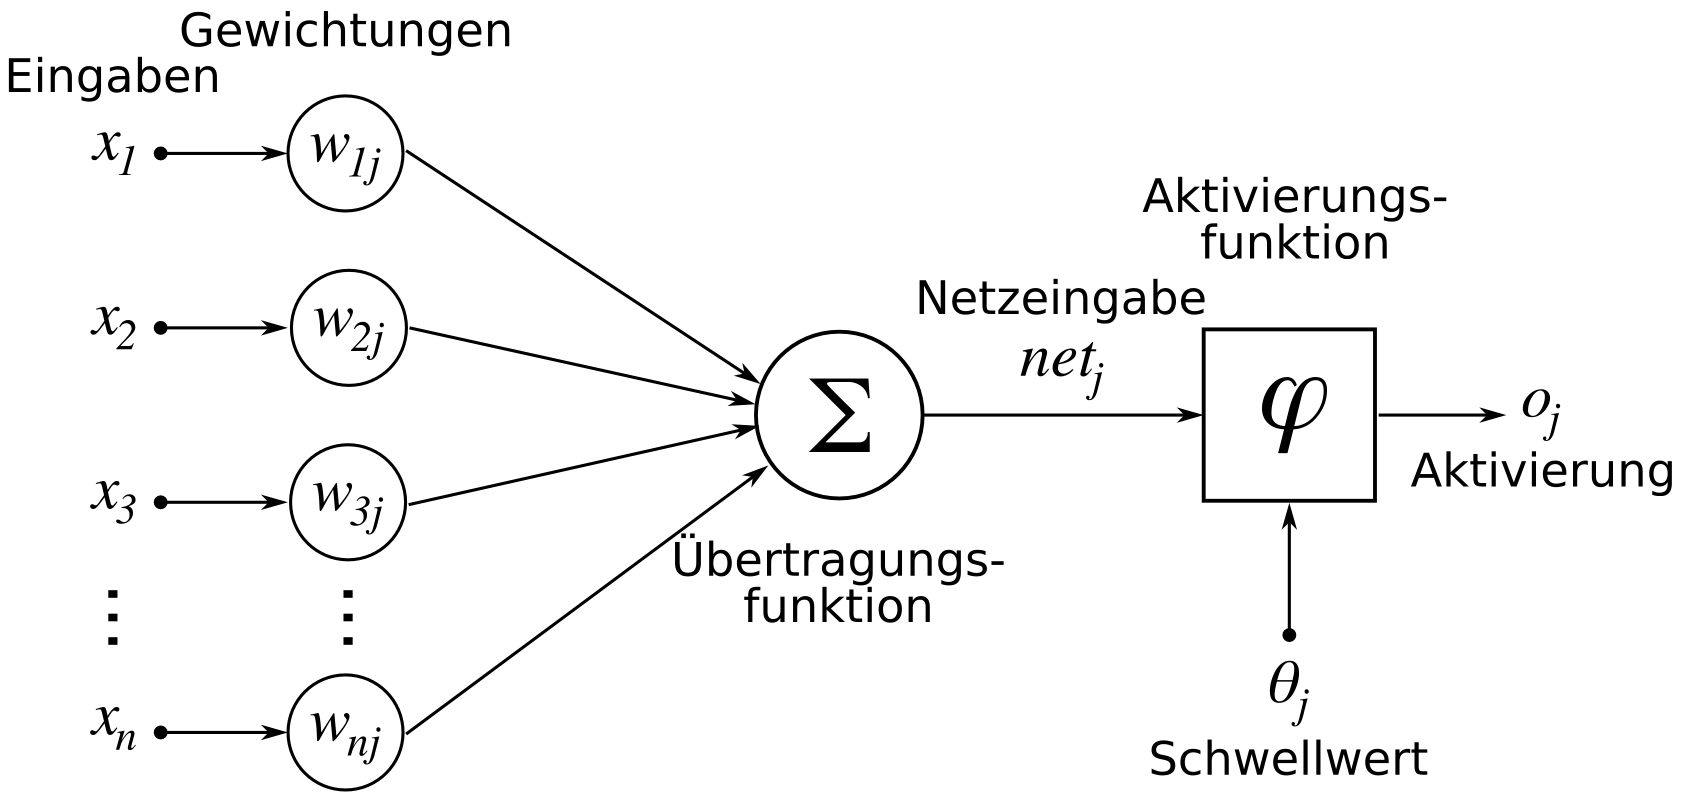
\includegraphics[height=0.6\textheight]{images/neural_net.png}
\end{figure}
\end{frame}

\begin{frame}
\frametitle{Neurónové siete, Strojové učenie}

\textcolor{red}{Gradientová metóda} pri odvodení tzv. ''delta-rule''

\def\rpartial{\textcolor{red}{\partial}}

\begin{align*}
\dfrac{\rpartial E_j}{\rpartial W_{jk}} (W_j) = \\
\sum_{p=1}^{t} (y^{(p)}_j - d^{(p)}_j)     \dfrac{\rpartial y^{(p)}_j} {\rpartial W_{jk}} (W_j)= \\
\sum_{p=1}^{t} (y^{(p)}_j - d^{(p)}_j)     f'(net_j^{(p)}) \dfrac{\rpartial \sum_{i=1}^{n} W_{ji} x_i^{(p)}}{\rpartial W_{jk}} (W_j)= \\
\sum_{p=1}^{t} (y^{(p)}_j - d^{(p)}_j)     f'(net_j^{(p)}) x_k^{(p)} \\
\end{align*}

\end{frame}

\subsection{Grafika, Počitačové siete}

\begin{frame}
\frametitle{Grafika, Počitačové siete (2)}
\begin{figure}
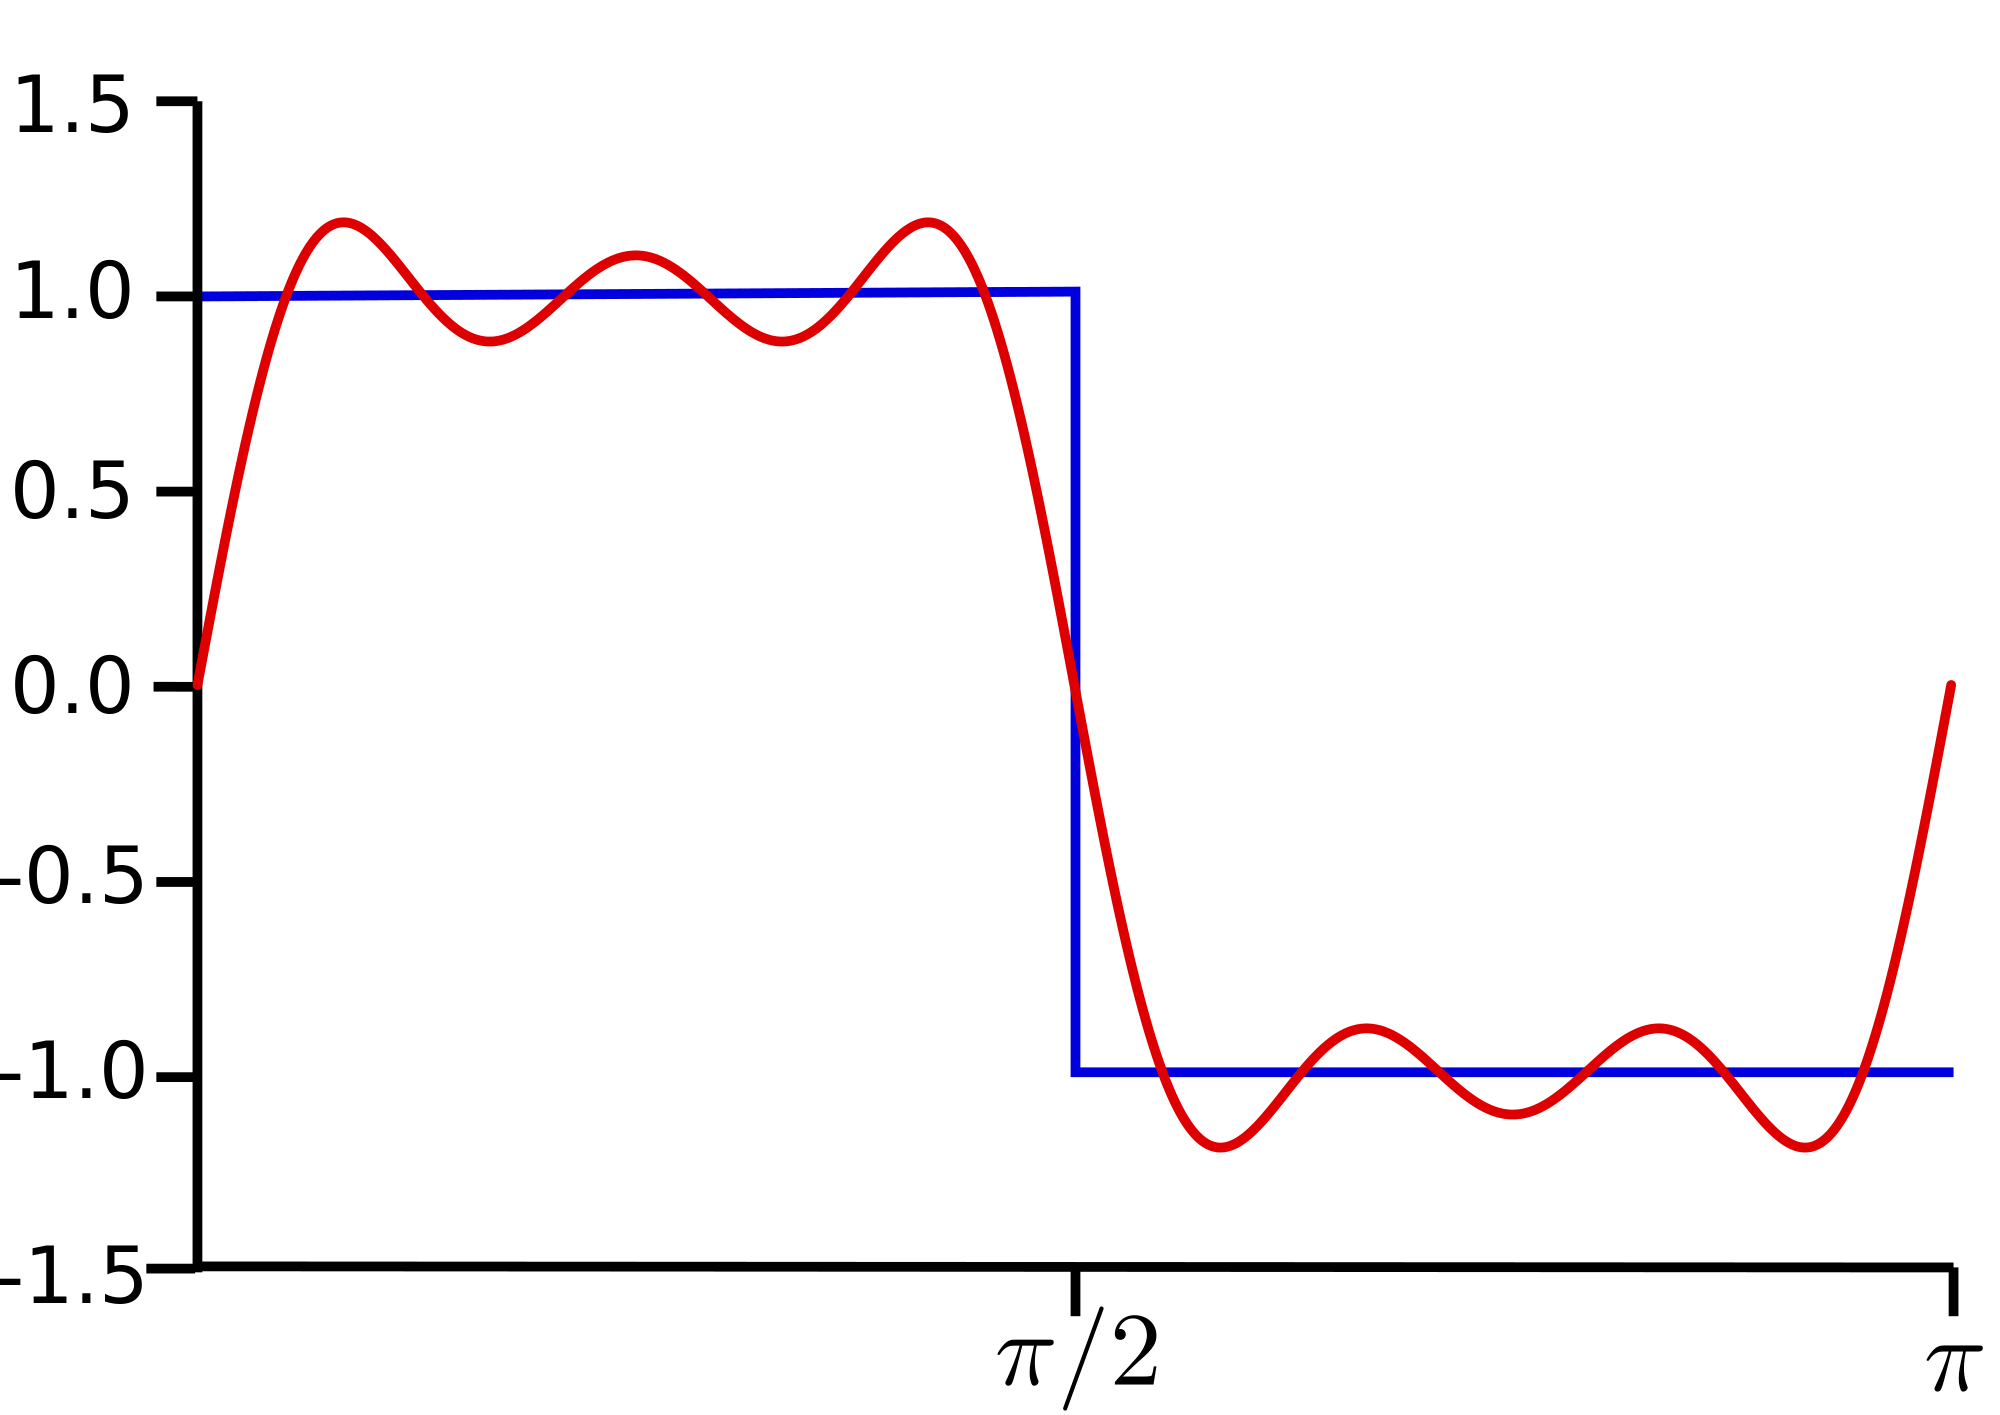
\includegraphics[height=0.8\textheight]{images/fourier_signal.png}
\end{figure}
\end{frame}


\begin{frame}
\frametitle{Grafika, Počitačové siete (2)}
\begin{block}{Fourierova transformácia}
$$F\{f(x)\} = F(u) = \int_{-\infty}^{+\infty} f(x) \cdot [\cos{2\pi ux} - i \sin{2\pi ux}] ~ dx$$
\end{block}
\end{frame}

\subsection{Kombinatorická analýza}

\begin{frame}
\frametitle{Kombinatorická analýza}
\pause
$$\sum_{k=0}^{n} k = 1 + 2 + \ldots + (n-1) + n \pause = \dfrac{n(n+1)}{2}$$
\pause
$$\sum_{k=0}^{n} k^2 = \pause \dfrac{n(n-1)(2n-1)}{6}$$
\pause
$$\sum_{k=0}^{n} k^3 = ?? \pause $$

meh, tu je všeobecný vzorec:

$$\sum_{n \geq 0} \textcolor{red}{k^m} x^n = (xD)^{\textcolor{red}{m}} \left(\dfrac{1}{1-x}\right)$$
\end{frame}

\begin{frame}
\frametitle{Kombinatorická analýza}
\begin{columns}[c] % The "c" option specifies centered vertical alignment while the "t" option is used for top vertical alignment

\column{.5\textwidth} % Left column and width
\textbf{Matalýza}
\begin{enumerate}
\item<1-> $ D f(x) = \lim_{\tilde{x} \to x} \dfrac{f(\tilde{x}) - f(x)}{\tilde{x} - x}$
\item<2-> $\int f(x) dx$
\item<3-> $\int f~Du = fg - \int Df ~g $
\end{enumerate}

\column{.5\textwidth} % Right column and width
\textbf{Kombat}
\begin{enumerate}
\item<1-> $ \Delta f (n) = f(n+1) - f(n)$
\item<2-> $\sum f(n) \delta n$
\item<3-> $\sum u ~ \Delta v = u v - \sum \Delta u ~ Ev$ ($E f(n) = f(n+1)$)
\end{enumerate}
\end{columns}
\end{frame}

\begin{frame}
\frametitle{Záver?}
\begin{itemize}
  \item funkcionálne rady, topológia (Teória programovania, Verifikácia prográmov (aj databázy))
  \item integrálny počet funkcií viacerých premenných (Moderná štatistika)
  \item differenciálne rovnice (ľubovoľná fyzikálna (aj grafická) simulácia)
  \item Taylorove rady = (obyčajné) generujúce funkcie (Kombinatorické štruktúry)
  \item \ldots
\end{itemize}
\end{frame}

\begin{frame}
\frametitle{Záver?}
\begin{figure}

\includegraphics[height=0.8\textheight]{images/let_calculus_flow.jpg}
\end{figure}
\end{frame}

\begin{frame}
\frametitle{Kam ďalej?}
\begin{itemize}
\item prečítajte si pozorne svoj študijný plán (najmä prerekvizity)
\pause
\item zvážte Matematickú analýzu (3) (gradient, differenciálne rovnice, etc.)
\pause
\item poznámky od Kamily ku MA(1) a (2): \url{http://ksp.sk/~kamila/ma/}
\pause 
\item možno aj Algebra (2) má význam \pause (však je to na štatniciach :D )
\pause
\item prezentáciu (a malý bonus pre aktívnych) najdete na mojej stránke: \url{ksp.sk/~askar}
\end{itemize}
\pause 

\begin{LARGE}
\begin{center}
\textbf{Ďakujem za pozornost!}

\end{center}
\end{LARGE}

\end{frame}

\end{document} 
